\documentclass{article}
\usepackage{graphicx}
\usepackage{listings}
\usepackage{flexisym}

\graphicspath{ {images/} }

\newcommand{\overbar}[1]{\mkern 1.5mu\overline{\mkern-1.5mu#1\mkern-1.5mu}\mkern 1.5mu}

\begin{document}

  \title{CS 321: Assignment 4}
  \author{Jared Wasinger}

  \maketitle

  \begin{enumerate}
		\item Give a regular expression $R$ such that $\overline{L(R)} = L((ab + aab)*b)$\\
			Want a regular expression: $(\Sigma^* \setminus \{ab, aab\})^*a$\\
			Let $C$ be the language described by $\Sigma^* \setminus \{ab, aab\} = $\\
			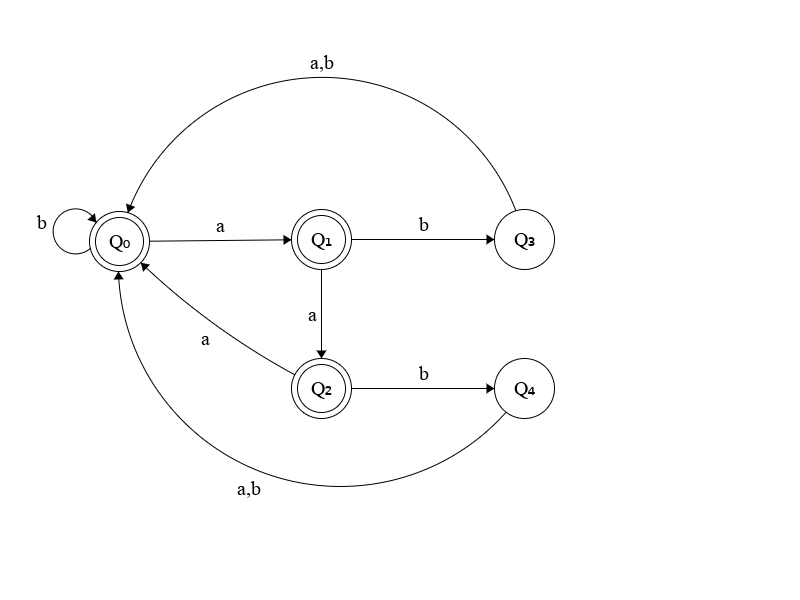
\includegraphics[width=\textwidth]{p1_C.png}\\
			\textbf{Reduce to regular expression}\\
			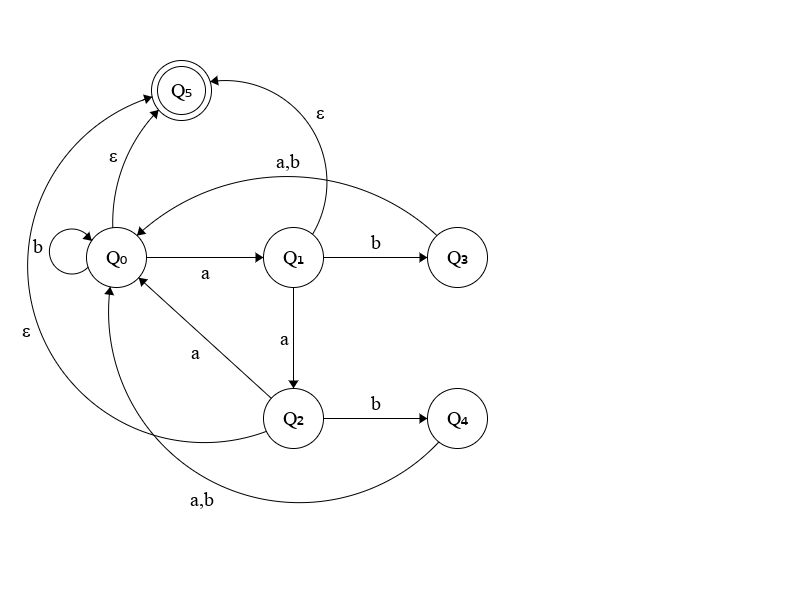
\includegraphics[width=\textwidth]{p1_C_reduced_1.png}\\
			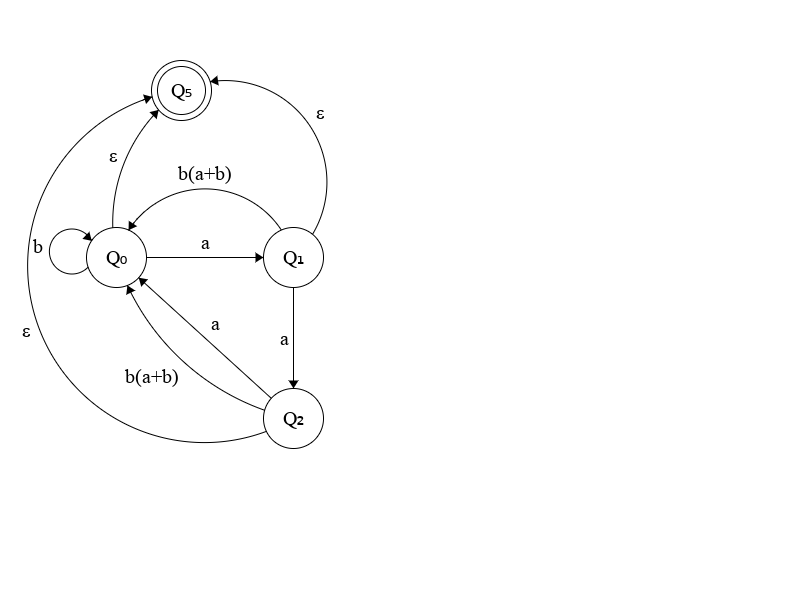
\includegraphics[width=\textwidth]{p1_C_reduced_2.png}\\
			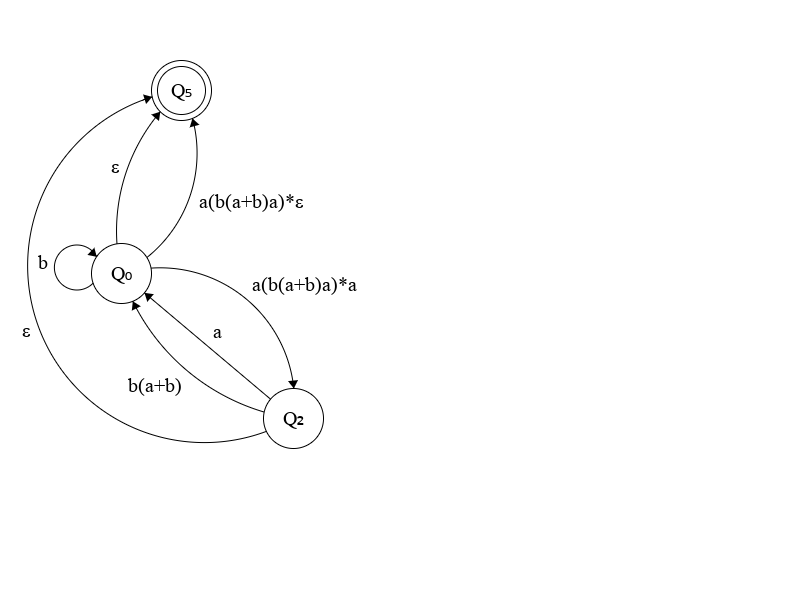
\includegraphics[width=\textwidth]{p1_C_reduced_3.png}\\
			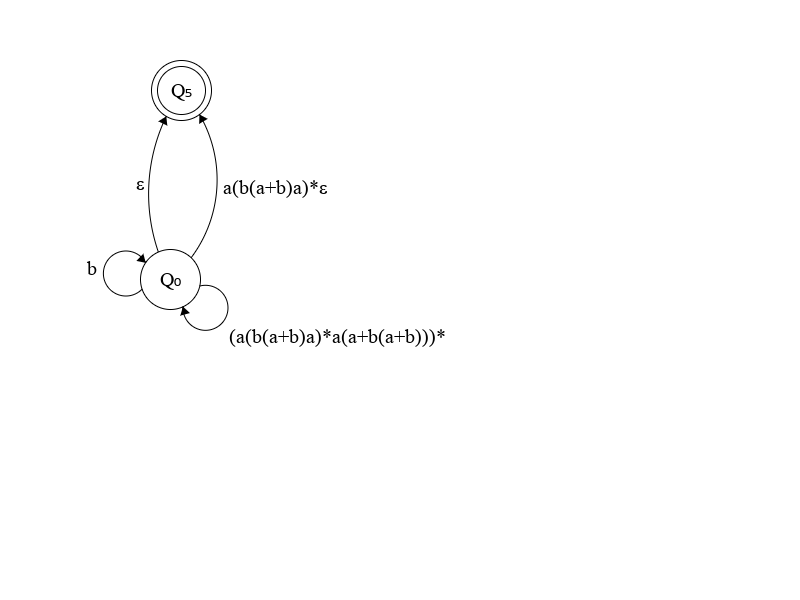
\includegraphics[width=\textwidth]{p1_C_reduced_4.png}\\

			\textbf{Regular Expression that describes C}: $a(b(a+b)a)^* + (a(b(a+b)a)^*a(a+b(a+b)))^* + b*$\\
			Complement of $L(R) = C*b = (a(b(a+b)a)^* + (a(b(a+b)a)^*a(a+b(a+b)))^* + b*)*a$

		\item Give a DFA equivalent to the following regular expression:\\
			$\epsilon + a(ba^*b + ba)^*b$\\
			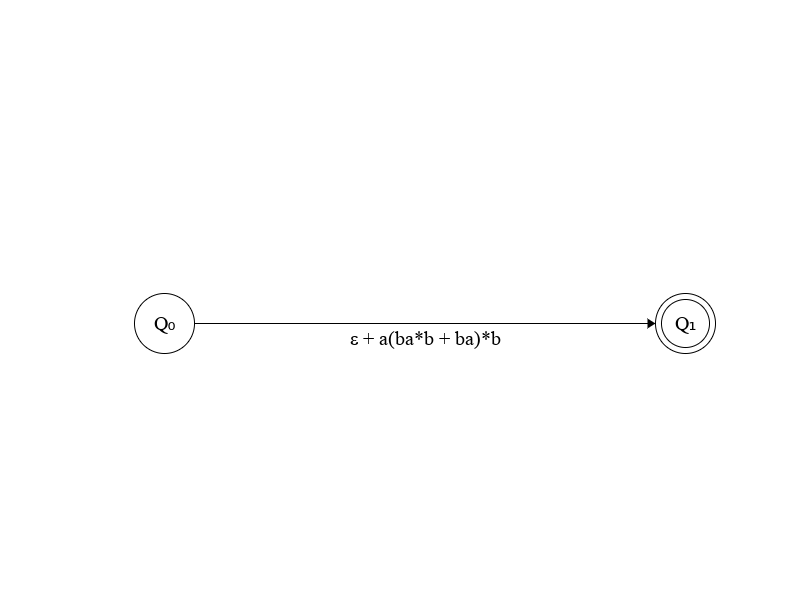
\includegraphics[width=\textwidth]{p2_1.png}\\
			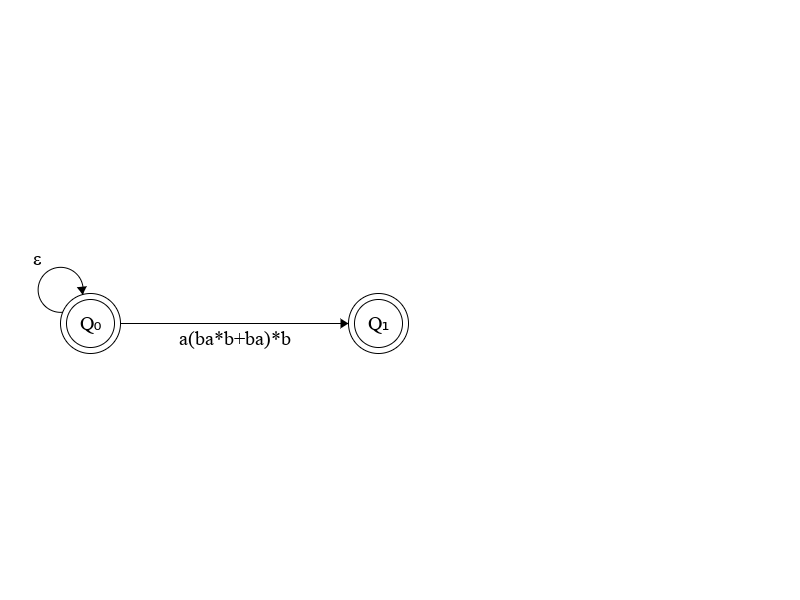
\includegraphics[width=\textwidth]{p2_2.png}\\
			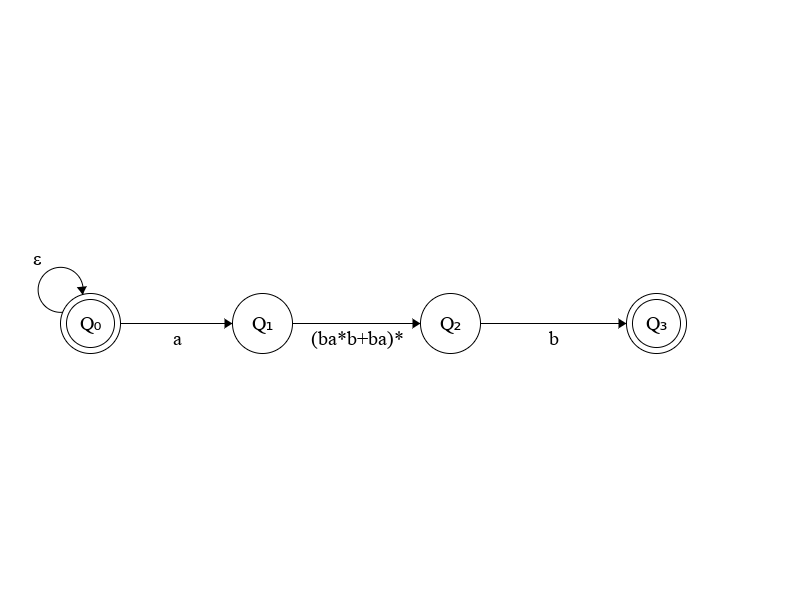
\includegraphics[width=\textwidth]{p2_3.png}\\
			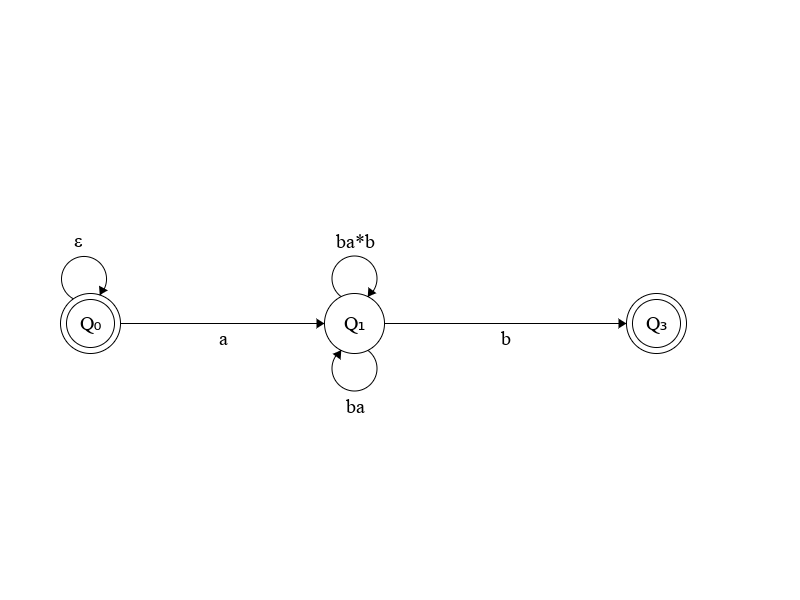
\includegraphics[width=\textwidth]{p2_4.png}\\
			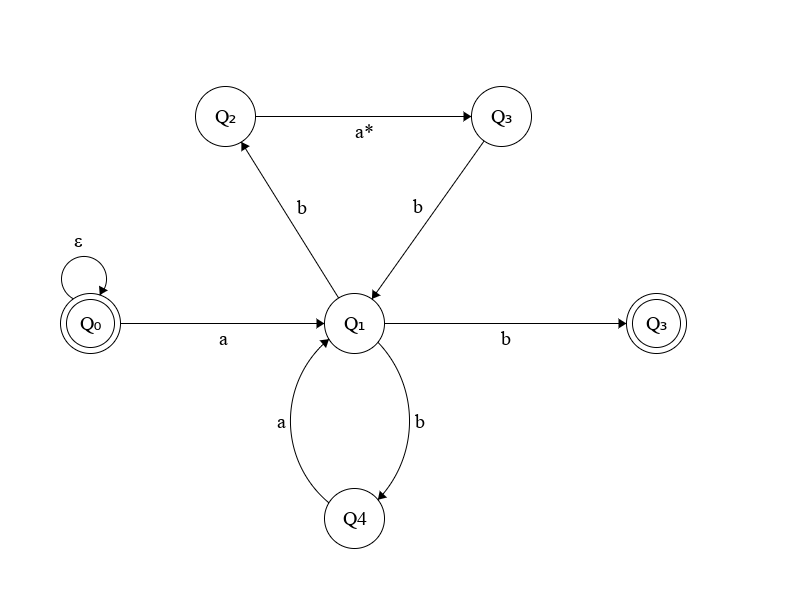
\includegraphics[width=\textwidth]{p2_5.png}\\
			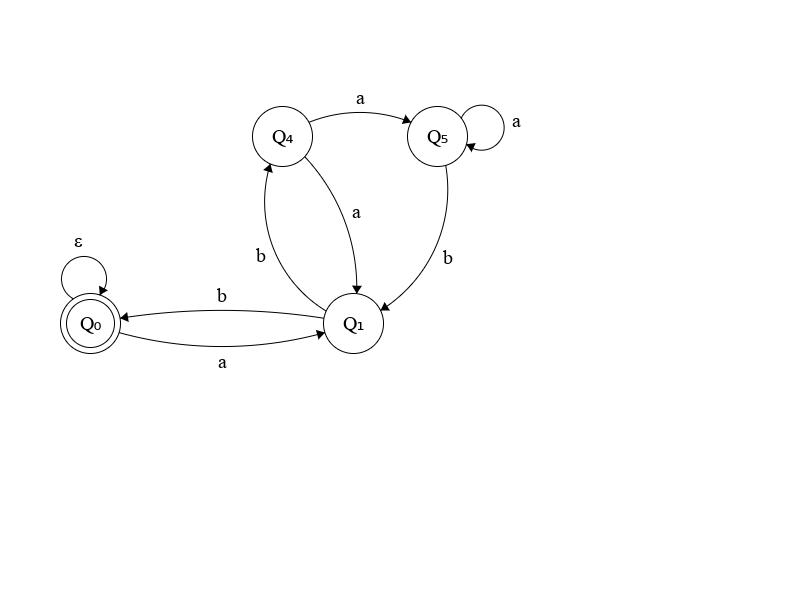
\includegraphics[width=\textwidth]{p2_6.png}\\

      DFA Transition table\\\\
      \begin{tabular}{ l | c | r | r }
        State & a & b & $\epsilon$ \\ \hline
        $\{q_0\}$ & $\{q_1\}$ & $\{\emptyset\}$ & $\{q_0\}$ \\

        $\{q_1\}$ & $\{\emptyset\}$ & $\{q_0, q_4\}$ & $\{\emptyset\}$\\

        $\{q_0, q_4\}$ & $\{q_1, q_5\}$ & $\{\emptyset\}$ & $\{\emptyset\}$ \\

        $\{q_1, q_5\}$ & $\{q_5\}$ & $\{q_1, q_4\}$ & $\{\emptyset\}$ \\

        $\{q_1, q_4\}$ & $\{q_5\}$ & $\{q_0, q_4\}$ & $\{\emptyset\}$ \\

      \end{tabular}

			\textbf{Convert NFA to DFA}\\
		\item $A = \{w \in \{a,b\}^* | $10th character from the end of $w$ is $b\}$. Prove that if DFA $M$ has $L(M)$, then $M$ has at least 1024 states.\\
			\textbf{Solution:}\\
			$let X = \{\delta^*(s,w) | w \in \{a,b\}^* | len(w) = 10\}$\\
			\begin{enumerate}
				\item First character is 'b'\\
				\item Each subsequent character is 'a' or 'b'\\
				\item Total number of states in $X$ = $\sum_{i=0}{i<9}2^i + 1 = 1024$
			\end{enumerate}
			\textbf{Contrapositive}\\
			\begin{enumerate}
				\item Suppose M has fewer than 1024 states.
				\item In order for $M$ to have $L(A)$, there must be repeated states in M
				\item However, if states are repeated, then by the Pigeonhole principle, there must be cycles in M.
				\item By the definition of a cycle, two strings of differing length will end up in the same final state.  A DFA with less than 1024 states will 'forget' where it is at in the string it is reading in.
				\item Let $j$ be an integer greater than 10.
				\item $\delta(s, b(a+b)^{j-1}) \in F(M)$ - a string where $b$ is not the 10th to the last character will be accepted by $M$, and rejected by $A$.
			\end{enumerate}
	\end{enumerate}
\end{document}
